\documentclass[12pt]{article}
\usepackage{amsmath}
\usepackage{array}
\usepackage{cancel}
\usepackage[thinc]{esdiff}
% \usepackage{gensymb}
\usepackage{geometry}
\usepackage{graphicx}
\usepackage{pgfplots}
\usepackage{siunitx}
\usepackage{wrapfig}
\usepackage{xcolor}

\title{Homework \#9, 4B}
\author{Donald Aingworth IV}
\date{March 19, 2025}

\pgfplotsset{width=8cm,compat=1.9}
\usepgfplotslibrary{external}
% \tikzexternalize

\renewcommand\thesubsection{\alph{subsection}}
\newcommand{\proj}{\text{proj}}

\begin{document}

\DeclareSIUnit{\mile}{mi}
\DeclareSIUnit{\gal}{gal}
\DeclareSIUnit{\foot}{ft}
\DeclareSIUnit{\hour}{h}
\DeclareSIUnit{\rad}{rad}
\DeclareSIUnit{\unit}{u}
\DeclareSIUnit{\dyne}{dyn}

\maketitle

\pagebreak
\section{Problem 2}
\begin{wrapfigure}{r}{0.25\textwidth}
    \vspace{-30pt}
    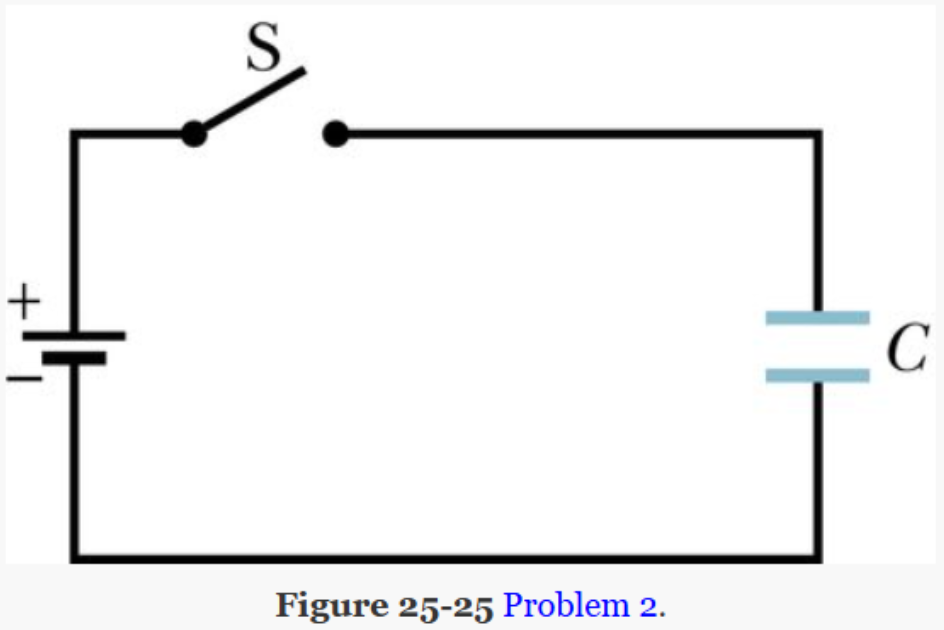
\includegraphics[width=0.25\textwidth]{picture_1.png} 
    % \label{fig:wrapfig}
\end{wrapfigure}
The capacitor in Fig. 25-25 has a capacitance of $25 \unit{\micro\farad}$ and is initially uncharged. 
The battery provides a potential difference of 120 V. 
After switch S is closed, how much charge will pass through it?

\subsection*{Solution: 3 mC}
We have an equation for this. 
For the capacitor to become fully charged, the charge that is the answer must pass into the capacitor and through the switch.
We have an equation for charge to enter a capacitor from voltage.
\begin{align*}
    q   &=  CV
        =   (25 \times 10^{-6}) * 120
        =   3000 \times 10^{-6} \unit{\coulomb}
        =   \boxed{\boxed{3 \unit{\milli\coulomb}}}
\end{align*}

\pagebreak
\section{Problem 4}
The plates of a spherical capacitor have radii 38.0 mm and 40.0 mm. 
(a) Calculate the capacitance. 
(b) What must be the plate area of a parallel-plate capacitor with the same plate separation and capacitance?

\subsection{Solution: }
We 

\end{document}